\chapter{State of the Art} \label{sec:cap2}

\section{Introduction to the \acs{ITER} Project}

The \ac{ITER} project is an international collaboration aimed at demonstrating the feasibility of nuclear fusion as a large-scale and carbon-free source of energy. It is being constructed in Cadarache, France, and involves 35 countries, including the European Union, the United States, China, India, Japan, Russia, and South Korea. The project aims to build the world's largest tokamak reactor, which will use magnetic confinement to achieve controlled nuclear fusion.

Inside the tokamak, plasma will be heated to extremely high temperatures, allowing hydrogen isotopes to fuse and release energy. The reactor is designed to produce ten times more energy than it consumes, making it a potential game-changer in the field of energy production.

A \textit{Discharge} is a plasma operation in the tokamak, where the plasma is created and maintained for a certain period. Each discharge is characterized by various parameters, such as plasma current, inductance, density, radiated power or input power. When these parameters deviate from their expected values, it can indicate potential issues or anomalies in the reactor's operation.

A \textit{Disruption} is an event that occurs when the plasma becomes unstable and loses confinement, leading to a rapid cooling of the plasma and a loss of control. For this project, discharges are classified as either normal or anomalous.

A \textit{Campaign} is a set of discharges that are analyzed together. For this project, there are three campaigns available, each containing a different number of discharges.

A visual representation of the plasma current on several discharges is shown in \autoref{fig:plasma-current}. This figure illustrates the singular bathtub shape of non-disruptive discharges, whereas disruptive discharges show a more erratic and not consistent pattern.

\begin{figure}[H]
    \centering
    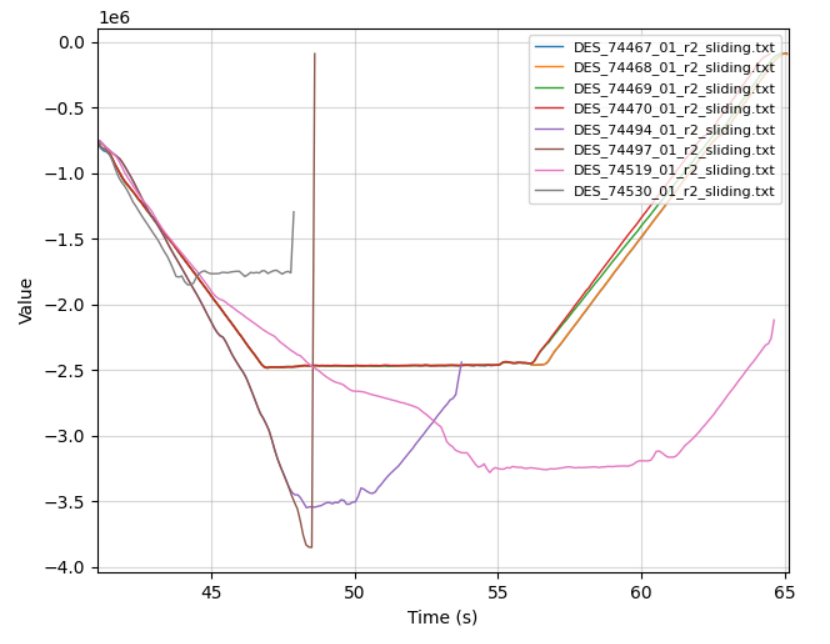
\includegraphics[width=0.8\textwidth]{plasma-current.png}
    \caption{Plasma current on disruptive and non-disruptive discharges}
    \label{fig:plasma-current}
\end{figure}

\section{Anomaly Detection in Nuclear Fusion}

Anomaly detection in nuclear fusion is crucial for ensuring the safe and efficient operation of reactors like \ac{ITER}. The complexity of the plasma behavior and the multitude of parameters involved make it challenging to monitor and control the system effectively. Anomalies can lead to disruptions, which can damage the reactor components and affect the overall performance.

To address this challenge, various machine learning techniques have been applied to analyze the data generated during discharges. These techniques aim to identify patterns and deviations in the data that may indicate potential anomalies. An early detection of these anomalies is essential to prevent disruptions and ensure the stability of the plasma, using gas injection to stop the nuclear fusion reaction before it causes damage to the reactor.

\section{Current implementation}

The current implementation is based on a \ac{SVM} model trained on historical discharge data. The model is designed to classify discharges as normal or anomalous based on the input parameters. The training process involves using labeled data, where each discharge is categorized as either normal or anomalous.

\ac{SVM} is a machine learning whose goal is to find the optimal hyperplane that separates the data into different classes \autocite{6524743}. On the training phase, the model receives entire discharges as input, and the category of the discharge. The model divides data in windows of 32 milliseconds, and extracts the mean value and the \ac{FFT} of each window.
